\documentclass[11pt,a4paper]{article}
\usepackage[margin=25mm]{geometry}
\usepackage{amsmath,amssymb,amsthm,graphicx,booktabs,hyperref,xcolor}
\definecolor{jade}{HTML}{12665E}
\hypersetup{colorlinks=true,linkcolor=jade,citecolor=jade,urlcolor=jade,pdftitle={How a reversible transition amplifies apparent entropy production},pdfauthor={Anonymous}}
\newtheorem{theorem}{Theorem}
\newtheorem{corollary}[theorem]{Corollary}
\newtheorem{lemma}[theorem]{Lemma}
\newtheorem{proposition}[theorem]{Proposition}
\newcommand{\av}[1]{\left\langle #1\right\rangle}
\newcommand{\KL}{\mathrm D}
\newcommand{\F}{\mathrm F}
\newcommand{\B}{\mathrm B}
\newcommand{\pos}[1]{\left[#1\right]_+}
\newcommand{\dd}{\,\mathrm d}
\setlength{\emergencystretch}{2em}
\title{\bfseries How a reversible transition amplifies apparent entropy production\\[4pt]
\large A counterexample to the uncorrected waiting-time inequality of Harunari, Fiore and Barato, and the sharp correction for blocks of waits}
\author{Anonymous\\[3pt]{\small DOI \href{https://doi.org/10.5281/zenodo.24529102}{10.5281/zenodo.24529102}}}
\date{November 2026}
\begin{document}
\maketitle
\begin{abstract}
Harunari, Fiore and Barato (HFB) proposed estimating the entropy production of a periodically driven system from histograms of the waiting times between visible jumps, recorded once with the driving protocol and once with the protocol reversed, without recording the phase of the drive. They proved that the estimate minus a correction term $X$ is a lower bound on entropy production and left open whether the uncorrected estimate is one as well. We show that it is not, and that its excess is unbounded. In a smooth three-state model with zero period-averaged current on every edge, equal event rates in both experiments and fixed entropy production $4\pi/5$, the estimate grows linearly with the rate of a reversible transition. An exact rational certificate proves that it exceeds 31 times the entropy production at one finite rate, and a certified lag-bin bound raises the factor above 145. The failure persists when every microscopic jump is recorded, and under a small constant cycle affinity, which in numerical solutions makes the system pump a net current. For general finite driven networks we extend HFB's correction to records of $m$ consecutive waits: the block estimate exceeds the phase-resolved bound by at most $X/m$, where $X$ needs only the phase histogram of each kind of visible event, and the coefficient of $X/m$ cannot be lowered. In the example we determine the block estimate in every scaling regime, from single waits to blocks that span many periods.
\end{abstract}

\section{Introduction}
This section states the problem, explains why it matters, summarises what was known and what is new, and gives a roadmap.

\paragraph{The problem.} Small driven systems, such as molecular motors, ion channels and colloids in moving traps, turn part of the energy they receive into heat. The rate of this \emph{entropy production} is a basic thermodynamic quantity, but in experiments most internal states are hidden: one sees only a few transitions, for example a bead hopping between two wells, together with the times at which they occur. A large literature therefore derives \emph{lower bounds} on entropy production from the statistics of visible jumps and of the waiting times between them \cite{vandermeer,harunari2022,skinner,martinez,snippets}. If the waiting-time statistics look different when time runs backwards, the system must dissipate at least a computable amount.

Many experiments are driven periodically, by an oscillating field or trap. Harunari, Fiore and Barato \cite{hfb} extended the waiting-time method to this setting. Their estimator, here called $S_1$, uses two experiments, one with the driving protocol and one with the protocol run backwards, and compares the two histograms of waiting times between consecutive visible jumps. It does not need a clock synchronised to the drive, which makes it practical. HFB proved the inequality $\sigma\geq S_1-X$, where $\sigma$ is the entropy production and $X\ge0$ is a correction that requires the phase of individual events. In their case study the uncorrected estimate stayed below $\sigma$, and they wrote that their numerics ``indicate the possibility of the inequality $\sigma\ge\hat\sigma$'' (their $\hat\sigma$ is our $S_1$) while stressing that this was restricted to one model \cite[Sec.~VI]{hfb}. They also observed that when the net current vanishes the estimate is often ``numerically compatible with zero'' and suggested that the method gives little information for systems without a net current.

\paragraph{What was known.} A related phase-blind statistic proposed by Maier, Deg\"unther, van der Meer and Seifert \cite{maier} uses only the forward experiment. An earlier Evidence Press release \cite{ep} refuted that forward-only conjecture. For protocols that are symmetric under time reversal the forward-only statistic coincides with HFB's $S_1$, and Section~6 of that release reported a numerical overshoot of about $10\%$ in such a protocol, which already bore on HFB's question; it was not certified. That release listed ``estimators that use the reversed-protocol experiment'' among those unaffected by its counterexamples. This remains true of the phase-resolved estimator and of HFB's corrected inequality $\sigma\ge S_1-X$, which no example can violate; the present paper shows that it is not true of the uncorrected estimate $S_1$.

\paragraph{What is new.}
\begin{itemize}
\item \emph{An analytic counterexample with unbounded excess} (Theorem~\ref{th:finite}). A smooth three-state model with zero period-averaged currents, matched event rates and fixed $\sigma=4\pi/5$ has $S_1$ growing linearly in the rate $R$ of one reversible transition; an exact rational certificate gives $S_1>31\sigma$ at one rate, and a certified lag-bin bound gives $S_1>145\sigma$ (Proposition~\ref{prop:bins}). The example directly contradicts the expectation that zero net current makes the estimate small.
\item \emph{Robustness.} The failure survives complete observation of all microscopic jumps (Section~\ref{sec:high}) and a small constant cycle affinity (Corollary~\ref{cor:pump}); numerically the biased model then pumps a net current, and the overshoot persists up to the largest affinity tested.
\item \emph{The sharp correction for blocks} (Theorems~\ref{th:block} and~\ref{th:sharp}). For any finite driven network, a record of $m$ consecutive waits overstates the phase-resolved bound by at most $X/m$. At $m=1$ this is HFB's corrected inequality, their Eq.~(26); the new content is the extension to blocks, a simple criterion for when the uncorrected estimate is safe, and the proof that the coefficient of $X/m$ is optimal.
\item \emph{A complete scaling picture in the example} (Section~\ref{sec:sharp} and the appendices): how many consecutive waits are needed before the phase-blind block estimate recovers the true dissipation, with a transition at $m$ of order $R^{2/3}$ where the waits start to reveal whether the drive is rising or falling.
\end{itemize}

\paragraph{Roadmap.} Section~\ref{sec:setup} defines the experiments, the estimator and the phase-resolved bound. Section~\ref{sec:finite} gives the counterexample and its certificates, including the pumped-current variant. Section~\ref{sec:high} identifies the high-activity limit and treats complete observation. Section~\ref{sec:block} proves the block correction and the safety criterion; Section~\ref{sec:sharp} proves that its coefficient is sharp and tabulates the scaling regimes. Section~\ref{sec:discussion} relates the results to earlier work and states the practical consequences and limits. Appendices~\ref{app:short} and~\ref{sec:macro} contain the asymptotic proofs and Appendix~\ref{app:bins} the finite-rate certificates.

Entropy is measured in units of $k_{\rm B}$ with natural logarithms. Rates are per driving period in the example. The physical quantity is the entropy production of the driven Markov system as defined in HFB Eq.~(2); an apparatus may dissipate additional energy to operate the controls.

\section{Setting: event sampling, reversal and the estimator}\label{sec:setup}
This section fixes notation for the two experiments and defines HFB's estimator and the phase-resolved bound against which it is compared.

Let $k_{xy}(s)$ be the transition rates of a continuous-time Markov jump process on a finite connected graph whose edges are bidirected. The rates are continuous and periodic in the phase $s$ with period $T$, bounded above, and bounded away from zero on the edges. The \emph{forward experiment} $\F$ uses $k^\F=k$; the \emph{backward experiment} $\B$ runs the protocol in reverse, $k^\B_{xy}(s)=k^\F_{xy}(-s)$, with phases taken modulo $T$ (HFB Eq.~(13)). Each experiment is observed in its own periodic state $\pi_E(s)$, $E\in\{\F,\B\}$. Write $\av{f}=T^{-1}\int_0^T f(s)\dd s$. The physical entropy production rate is
\begin{equation}
\sigma=\av{\sum_{x,y}\pi_{\F,x} k_{xy}^\F\log(k_{xy}^\F/k_{yx}^\F)} ;
\label{eq:epr}
\end{equation}
the period integral removes the derivative of the system's Shannon entropy.

\paragraph{Visible events.} The observer sees a nonempty set of directed edges closed under reversal, and records each such jump with its time. A visible directed edge is called a \emph{mark}; marks are written $i,j$, and $\bar i$ is the reverse of $i$. For $i=(x,y)$ the event intensity is $r^E_i(s)=\pi_{E,x}(s)k^E_{xy}(s)$, and the visible activity (events per unit time) is $K_E=\sum_i\av{r_i^E}$. A typical visible event, sampled by counting events in a long record, has joint phase-and-mark law $\mu_E(\dd s,i)=r_i^E(s)\dd s/(TK_E)$ on one period, with mark marginal $\nu_E(i)$. This is the event-sampled (Palm) law: the sequence of phases, marks and waiting times seen from a typical event is stationary in the event index.

\paragraph{The estimator.} Write $f^E_{j|i}(u|s)$ for the density that, after mark $i$ at phase $s$, the next visible event is mark $j$ after a waiting time $u$. Averaging over the phase of the first event under $\mu_E(\dd s|i)$ gives the phase-blind density $\psi^E_{j|i}(u)$; summed over $j$ and integrated over $u$, it has mass one. HFB's estimator \cite[Eq.~(14)]{hfb} is
\begin{equation}
 S_1=K_\F\sum_{i,j}\nu_\F(i)\int_0^\infty
 \psi^\F_{j|i}(u)\log\frac{\psi^\F_{j|i}(u)}{\psi^\B_{\bar i|\bar j}(u)}\dd u .
\label{eq:est}
\end{equation}
The denominator describes the reversed pair: it starts at $\bar j$ and ends at $\bar i$. (HFB's normalisation of the phase density in their Eq.~(11) carries an extra factor $T^{-1}$; we use unit-mass conditional densities throughout, which is what the estimator requires.) The question is whether $S_1\le\sigma$ for every network and every set of visible marks.

\paragraph{The phase-resolved bound.} If the observer also records the phase of the first event, the natural comparison is between $f^\F_{j|i}(u|s)$ and the reversed backward kernel at the reflected phase of the second event. The \emph{phase-resolved rate} $\sigma_{\cal L}$ is $K_\F$ times the forward event expectation of
\begin{equation}
 \log\frac{f^\F_{j|i}(u|s)}{f^\B_{\bar i|\bar j}(u|-s-u)} .
 \label{eq:sigmaL}
\end{equation}
This is HFB's $\sigma_{\cal L}$ \cite[Eq.~(24)]{hfb}, and $\sigma_{\cal L}\le\sigma$ by data processing on path probabilities \cite{hfb,maier}. HFB's correction $X$ is defined in Eq.~\eqref{eq:x} below.

\section{A finite counterexample with no pumped current}\label{sec:finite}
This section constructs the counterexample, proves an explicit lower bound on $S_1$, and records the finite-rate certificates and a current-carrying variant.

\paragraph{The model.} Use three states: a hidden state $0$ and two ``twin'' states $+$ and $-$. Write $\theta=2\pi t$ with unit period, $h=4/5$, and
\begin{align}
 a(t)&=2\pi(1+h\sin 2\theta),&
 b(t)&=2\pi(1-h\sin 2\theta),&
 q(t)&=1+\tfrac{16}{17}\cos\theta.\label{eq:rates}
\end{align}
State $0$ jumps to each twin at rate $a/2$; each twin returns to $0$ at rate $b$. The two twins exchange at rate $Rq$ in both directions, with a large constant $R>0$. We call the twin--twin edge the \emph{reporter} and the four edges touching $0$ the \emph{slow edges}. At first only the reporter is visible; its two directions are the marks $(+,-)$ and $(-,+)$. All rates are smooth and strictly positive. The slow edges open and close the twins twice per period; the reporter rate varies once per period and is even in the phase, $q(-t)=q(t)$.

\begin{theorem}\label{th:finite}
The forward and backward experiments both have visible activity $R/2$ and equal frequencies of the two reporter directions. Every edge current averages to zero over a period, and at every phase the frozen rates satisfy detailed balance. For every $R>0$,
\begin{equation}
  \sigma=\frac{4\pi}{5},\qquad S_1\ \geq\ R\pos{\frac{17}{600}-\frac{2C}{R}}^2,
  \qquad C=\frac{18\pi}{5}+\frac{32\pi}{17}.
\label{eq:cert}
\end{equation}
In particular $S_1>78$ and $S_1/\sigma>31$ at $R=10^5$, where $\sigma<2.515$. The ratio $S_1/\sigma$ is unbounded as $R\to\infty$.
\end{theorem}

\begin{proof}
Let $p_E$ be the total probability of the twins. The exchange of $+$ and $-$ is a symmetry, so each twin has probability $p_E/2$. In the forward experiment $p'_\F=a-(a+b)p_\F$. Since $a+b=4\pi$ is constant, direct substitution gives the unique periodic solutions
\[
 p_\F=\tfrac12+\tfrac h4(\sin 2\theta-\cos 2\theta),\qquad
 p_\B=\tfrac12-\tfrac h4(\sin 2\theta-\cos 2\theta).
\]
Fourier orthogonality gives $\av{p_E q}=1/2$, so $K_E=R\av{p_Eq}=R/2$, with the two directions equally frequent. The reporter carries zero current pointwise, and each slow edge carries $p'_\F/2$ towards the twins, with zero mean. The frozen chain satisfies detailed balance with weights proportional to $(1,a/(2b),a/(2b))$.

Equation~\eqref{eq:epr} gives $\sigma=\av{p'_\F\log(a/b)}$, since the constant $-\log 2$ integrates to zero against $p'_\F$. For $0<h<1$ put $z=(1-\sqrt{1-h^2})/h$. The first sine coefficient of $\log[(1+h\sin x)/(1-h\sin x)]$ is $4z$: write $1\pm h\cos y=(1\pm2z\cos y+z^2)/(1+z^2)$, expand $\log(1\pm ze^{iy})$, and shift $y=x-\pi/2$. As $p'_\F=\pi h(\cos 2\theta+\sin 2\theta)$, we obtain $\sigma=2\pi(1-\sqrt{1-h^2})=4\pi/5$.

\emph{Reduction to one pair law.} In either experiment the exchange symmetry makes the two-by-two kernel of (next mark given current mark) have equal diagonal and equal off-diagonal entries, independently of the starting direction. Reversing a pair preserves whether its direction repeats or alternates and preserves its waiting time. With equal mark frequencies, Eq.~\eqref{eq:est} therefore equals $K_\F$ times the relative entropy between the forward and backward laws of (repeat or alternate, waiting time) at a typical reporter event, each in its own chronological order. Independently draw $W\sim{\rm Exp}(R)$ and record whether the next reporter event occurs before $W$. The probability of this binary outcome is $M_E=\mathbb E_E e^{-R\tau}$, where $\tau$ is the waiting time. Relative entropy cannot increase under this reduction, and Pinsker's inequality in nats gives
\[
 S_1\geq 2K_\F(M_\F-M_\B)^2 .
\]

\emph{Freezing the race.} After a reporter jump at phase $s$ the system is in a twin; the phase density of reporter jumps of either direction is $2p_E(s)q(s)$ on the unit period. Compare the true race with a frozen one in which the reporter rate stays $Rq(s)$ and the system cannot leave the twins; its success probability is $q(s)/(1+q(s))$. The two races differ only if a slow exit occurs before $W$, which has probability at most $\|b\|_\infty\mathbb E W=\|b\|_\infty/R$ (any path with an exit, including one that later re-enters, is counted as a failure of the coupling), or if the time-dependent and frozen reporter clocks disagree before $W$, which has probability at most $R\|q'\|_\infty\mathbb E W^2/2=\|q'\|_\infty/R$. The same bounds hold in the backward experiment, because $q$ is even. Hence
\begin{equation}
 |M_E-M_E^\infty|\leq C/R,\qquad
 M_E^\infty=2\av{p_E q^2/(1+q)} ,\label{eq:race}
\end{equation}
with $\|b\|_\infty=18\pi/5$ and $\|q'\|_\infty=32\pi/17$, so $C=\|b\|_\infty+\|q'\|_\infty$ and $|M_\F-M_\B|\ge |M^\infty_\F-M^\infty_\B|-2C/R$.

\emph{The limiting gap.} The sine term of $p_E$ integrates to zero against any function of the even function $q$. Since $q^2/(1+q)=q-1+(1+q)^{-1}$, only the second cosine harmonic of $(1+q)^{-1}$ survives:
\[
 M_\B^\infty-M_\F^\infty
 = h\av{\frac{\cos 2\theta}{2+(16/17)\cos\theta}}
 =h\frac{17}{30}\left(-\frac14\right)^{\!2}=\frac{17}{600}.
\]
The middle equality uses the Poisson-kernel expansion of $(2+(16/17)\cos\theta)^{-1}$, whose mean is $17/30$ and whose $n$th cosine moment is $(17/30)(-1/4)^n$. Combining the bounds proves Eq.~\eqref{eq:cert}. Substituting $\pi<22/7$ at $R=10^5$ gives the stated finite inequalities in exact rational arithmetic ($S_1\ge 78.336$, and $S_1/\sigma\ge31.156$ using $\sigma\le88/35$). The bound is positive only for $R>1200\,C/17\approx1216$.
\end{proof}

\begin{figure}[ht]
\centering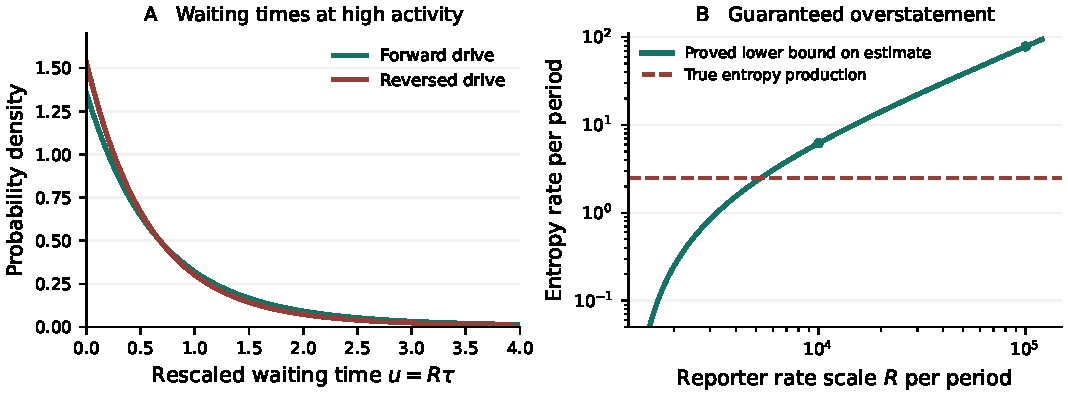
\includegraphics[width=.98\linewidth]{figure.pdf}
\caption{Left: the limiting densities $g_\F$ (forward drive) and $g_\B$ (reversed drive) of the rescaled waiting time between reporter events, Eq.~\eqref{eq:mix}; both integrate to one. Right, on logarithmic axes: the proved lower bound Eq.~\eqref{eq:cert} on the estimate and the true entropy production $4\pi/5$. The marked values of $R$ are $10^4$ and $10^5$.}
\end{figure}

\paragraph{Stronger finite certificates.} The one-bit test gives a short proof but discards most of the discrepancy. Several lag bins retain more. For a positive weight $w$ that depends on a pair of marks and the bin of its waiting time, the variational formula for relative entropy and $\log z\le z-1$ give $K\KL(P\|Q)\geq K[\mathbb E_P\log w-\mathbb E_Q(w-1)]$. Appendix~\ref{app:bins} lists the bins, weights and error terms and proves the following.
\begin{proposition}\label{prop:bins}
The certified lower bounds on $S_1$ in the table below hold. Here ``every jump visible'' denotes the one-gap estimator of Eq.~\eqref{eq:est} applied to the record of all six directed jumps, with its own activity $R/2+H$ (Section~\ref{sec:high}). At $R=10^5$ both exceed $366.44$, so $S_1/\sigma>145$ even with the rational upper bound $88/35$ on $\sigma$.
\end{proposition}
\begin{center}
\begin{tabular}{rrrl}\toprule
$R$ & One visible edge & Every jump visible & Method\\\midrule
750 & 2.74694 & 2.75561 & validated Fourier--Taylor enclosure\\
1\,000 & 3.65409 & 3.66107 & validated Fourier--Taylor enclosure\\
10\,000 & 21.62 & 21.62 & rational lag-bin bound\\
100\,000 & 366.44 & 366.44 & rational lag-bin bound\\\bottomrule
\end{tabular}
\end{center}
Entries are certified lower bounds rounded down; $\sigma=4\pi/5\approx2.5133$ throughout. Below $R\approx1216$ the analytic bound~\eqref{eq:cert} is vacuous, so the rows $R=750$ and $1000$ rest on the moderate-rate enclosure of Appendix~\ref{app:bins}. The smallest rate at which a violation is certified here is $R=750$, about $375$ reporter events per period; a floating-point binned lower bound in the code archive first exceeds $\sigma$ between $R=500$ (ratio $0.76$) and $R=750$ (ratio $1.15$).

\paragraph{How large is the excess in absolute terms?} The ratio is large because $\sigma$ is held fixed while the reporter speeds up. Per reporter event the numbers are small: the certified estimate is at least $0.0073$ nats per event at both $R=750$ and $R=10^5$, and its excess over $\sigma/K_\F$ is at least $6\times10^{-4}$ nats per event at $R=750$ and $0.0072$ nats at $R=10^5$, where $\sigma/K_\F\approx5\times10^{-5}$. HFB's own allowance is much larger: Eq.~\eqref{eq:xvalue} below gives $X/R=(1-\sqrt{17}/5)/2\approx0.088$, whereas $S_1/R\to0.0041$ (Theorem~\ref{th:slope}). The uncorrected estimate thus uses only a few per cent of the room that HFB's corrected inequality leaves, but that is enough to exceed $\sigma$ without bound.

\paragraph{Physical time scale.} One may instead keep the largest microscopic rate bounded by running the same process on a time axis stretched by $R$. The rates become $k_{xy}(t/R)/R$ and the period becomes $R$. Visible activity is then $1/2$ per unit time and entropy production is $4\pi/(5R)$ per unit time, whereas Eq.~\eqref{eq:cert} keeps the estimate per unit time bounded away from zero. In this description the counterexample is a slowly driven system: $\sigma$ vanishes in the quasi-static limit, but the phase-blind estimate does not.

\paragraph{A pumped current does not remove the effect.} The counterexample has no net current, and HFB found the estimator most informative for systems that pump one. A constant force on the reporter shows that the failure is not tied to zero current. For $f\in\mathbb R$ replace the reporter rates by $k_{+-}=Rq\,e^{f/2}$ and $k_{-+}=Rq\,e^{-f/2}$, leaving the slow rates unchanged. At every phase the product of rates around the cycle $0\to+\to-\to0$ divided by that around the reverse cycle is $e^f$, so $f$ is a constant cycle affinity.
\begin{corollary}\label{cor:pump}
Fix $R$ with $R\pos{17/600-2C/R}^2>4\pi/5$, for example any $R\ge5400$. There is $f_0>0$ such that the biased model satisfies $S_1(f)>\sigma(f)$ for $|f|<f_0$. At $R=10^5$ one may choose $f_0$ so that moreover $S_1(f)>30\,\sigma(f)$.
\end{corollary}
\begin{proof}
For any network, stationarity in the event index makes the second mark of a forward pair have law $\nu_\F$; expanding Eq.~\eqref{eq:est} then gives $S_1=K_\F[\KL(P\|\Theta Q)-\KL(\nu_\F\|\Theta\nu_\B)]$, where $P$ is the forward law of (first mark, second mark, waiting time), $Q$ the backward one and $\Theta$ maps $(i,j,u)$ to $(\bar j,\bar i,u)$ (Section~\ref{sec:block}). The deadline test of Theorem~\ref{th:finite} depends only on the waiting time and is invariant under $\Theta$, so data processing gives $S_1(f)\ge K_\F(f)\{\mathrm{kl}(M_\F(f),M_\B(f))-\KL(\nu_\F(f)\|\Theta\nu_\B(f))\}$, with $\mathrm{kl}$ the binary relative entropy and $M_E(f)$ the probability that the next visible event beats an independent ${\rm Exp}(R)$ deadline. At fixed $R$ every quantity here, and $\sigma(f)$, is a continuous function of $f$: the periodic states are the unique periodic solutions of irreducible linear equations whose coefficients depend continuously on $f$, and $M_E$ solves a periodic backward equation of the same kind. At $f=0$ the mark term vanishes and the right side is at least $2K_\F(M_\F-M_\B)^2\ge R\pos{17/600-2C/R}^2$, which exceeds $\sigma(0)=4\pi/5$ by hypothesis (at $R=5400$ it is at least $2.60$ in exact arithmetic with $\pi<22/7$), and exceeds $31\,\sigma(0)$ at $R=10^5$. Continuity gives the claim. The same argument applied to the weighted lag-bin tests of Proposition~\ref{prop:bins} gives the conclusion also at $R=750$ and $R=1000$.
\end{proof}
Numerically the biased model pumps a nonzero mean current for $f\ne0$, and the overshoot persists well away from $f=0$. At $R=1000$, with $13$ lag bins and marks retained (a floating-point lower bound on $S_1$; two phase meshes agree to a relative $10^{-5}$):
\begin{center}
\begin{tabular}{rrrrr}\toprule
$f$ & mean net current $0\to+$ & $\sigma(f)$ & lower bound on $S_1$ & ratio\\\midrule
0 & 0 & 2.5133 & 3.856 & 1.53\\
0.25 & 0.163 & 2.5539 & 3.827 & 1.49\\
0.5 & 0.320 & 2.6734 & 3.744 & 1.40\\
1 & 0.605 & 3.1178 & 3.444 & 1.10\\\bottomrule
\end{tabular}
\end{center}
Currents and $\sigma$ are per period. The model lies outside the family HFB studied; whether $S_1\le\sigma$ holds throughout their own three-state pump remains open, and their numerics suggest that it may.

\section{What survives at high activity}\label{sec:high}
This section identifies the exact large-$R$ slope of $S_1$, explains which feature of the rates a single wait can detect, and shows that observing every jump does not help.

For a typical reporter event let $U=R\tau$ be the rescaled waiting time. Define the two densities
\begin{equation}
 g_E(u)=2\av{p_E q^2 e^{-qu}},\qquad u\geq 0 .\label{eq:mix}
\end{equation}
Each is a mixture of exponentials: a rate $q(s)$ is drawn with the event-phase density $2p_Eq$, and the wait is exponential with that rate. Even a histogram that ignores directions can distinguish the protocols at high activity.

\begin{theorem}\label{th:slope}
For the one-edge observation, $S_1/R\to \tfrac12\KL(g_\F\|g_\B)>0$, where $\KL$ denotes relative entropy in nats. Numerical quadrature gives the slope $0.00407070$.
\end{theorem}

\begin{proof}
By the reduction in the proof of Theorem~\ref{th:finite}, $S_1/K_\F$ is the relative entropy between the forward and backward chronological laws of (repeat or alternate, waiting time) at a typical reporter event. Fix a starting direction, which fixes the post-jump twin, and work in rescaled time. Split according to whether the path visits $0$ before the next reporter event. With no such visit the next mark alternates, and its subprobability density is
\[
 H_{E,R}(u)=2\int_0^1 p_E(s)q(s)q(s+u/R)
 \exp\!\left\{-\int_0^u [q(s+v/R)+b_E(s+v/R)/R]\dd v\right\}\dd s,
\]
where $b_E$ is the exit rate in experiment $E$. It converges pointwise to $g_E(u)$. For $R\ge1$ it is bounded above by a constant times $e^{-u\min q}$ and below by a positive constant times $e^{-u(\max q+\max b)}$. Dominated convergence therefore applies to $H_{\F,R}\log(H_{\F,R}/H_{\B,R})$.

To control the paths that visit $0$, use the following augmented observation $O$: a flag recording whether $0$ is visited before the next reporter event; if not, the (alternating) mark and the waiting time; if so, the starting phase and the entire microscopic path up to the next reporter event. The type and waiting time are functions of $O$, so data processing bounds $S_1/K_\F$ above by the relative entropy of the two laws of $O$. That relative entropy equals $\int H_{\F,R}\log(H_{\F,R}/H_{\B,R})\dd u$ plus the forward expectation of the log likelihood ratio on the flagged event. On this event both experiments are compared at the same laboratory phase in chronological order; the common reporter rate cancels from the likelihood ratio, whose absolute logarithm is at most $c_0+c_1\tau+c_2N$ with constants independent of $R$, where $N$ counts slow jumps. This follows by multiplying the initial phase densities, the survival factors and the slow jump rates, all of which have bounded ratios. Reporter intervals partition physical time, so $\mathbb E_\F\tau=1/K_\F=2/R$, and $\mathbb E_\F N$ is the total slow activity divided by $K_\F$, which is $O(1/R)$; the flagged event itself has probability $O(1/R)$. The flagged contribution is therefore $O(1/R)$, which proves the upper limit. For the lower limit, the two laws of (type, waiting time) converge weakly to an alternating mark with waiting-time density $g_E$, and joint lower semicontinuity of relative entropy gives the opposite inequality. The unequal moments in Eq.~\eqref{eq:race} prove strict positivity.
\end{proof}

\paragraph{Which rates can a single wait distinguish?} The same argument applies to any smooth symmetric twin family with $q_\F=q_\B=q>0$ and bounded positive slow rates. Write $Z_E=\av{p_E q}$. The limiting density is $g_E(u)=\av{p_E q^2e^{-qu}}/Z_E$, the Laplace transform of $x\,\rho_E(\dd x)$, where $\rho_E$ is the distribution of the reporter rate $x=q(s)$ at a typical reporter event. These measures have compact support away from zero, so uniqueness of the Laplace transform gives $g_\F=g_\B$ precisely when $\rho_\F=\rho_\B$. Equal mean activities leave this distribution undetermined: one wait reveals how often each instantaneous rate is sampled, and the two protocols sample them differently.

\subsection*{Recording every microscopic transition}
The effect persists when the observer records the times and directions of all six directed jumps on the triangle and still uses the one-gap statistic. Each slow directed count has the same period average forward and backward: reversing the slow drive shifts it by a quarter period, and $p_E$ follows by the same shift. Forward and backward counts also agree under direction reversal, since the integrated current of every edge vanishes. The total slow activity is
\[
 H=\av{(1-p_\F)a+p_\F b}=2\pi(1-h^2/4).
\]
Set $K=R/2$ and $w=K/(K+H)$. With these matching mark frequencies, the estimator for complete observation, $S_1^{\rm all}$, equals $(K+H)$ times the relative entropy between the forward law of an ordered pair of successive marks with their gap and the reversed backward pair law.

Consider the binary test that \emph{both} marks are reporter jumps and the gap is shorter than an independent ${\rm Exp}(R)$ deadline. This test is invariant under reversal of the pair. Its probability in experiment $E$ is $w$ times the probability that, starting immediately after a reporter event, a reporter jump beats both a slow exit and the deadline. The frozen-race estimate in Eq.~\eqref{eq:race} applies with the same $C/R$ error, and Pinsker's inequality gives
\[
 S_1^{\rm all}\geq wR\pos{17/600-2C/R}^2 .
\]
In particular $S_1^{\rm all}>78$ at $R=10^5$. Complete detection of microscopic jumps therefore leaves the failure in place when the statistic discards the driving phase and cuts the record into one-gap comparisons.

\section{A correction for blocks of consecutive waits}\label{sec:block}
This section generalises HFB's corrected inequality from single waits to blocks of $m$ waits, for any finite driven network, and derives a criterion under which the uncorrected estimate is safe.

Let $P_m^E$ be the event-sampled law of $m$ successive waiting times and their $m+1$ marks in experiment $E$. The reversal map $\Theta$ reverses the order of both sequences and reverses every mark; on a single mark it maps $i$ to $\bar i$, and on a phase and mark it acts by $(s,i)\mapsto(-s,\bar i)$. The same symbol applied to a measure denotes its image. Define
\begin{align}
 S_m&=\frac{K_\F}{m}\{\KL(P_m^\F\|\Theta P_m^\B)
                       -\KL(\nu_\F\|\Theta\nu_\B)\},\label{eq:block}\\
 X&=K_\F\{\KL(\mu_\F\|\Theta\mu_\B)-\KL(\nu_\F\|\Theta\nu_\B)\}.\label{eq:x}
\end{align}
Both differences are nonnegative by marginalisation. For $m=1$, expanding the pair density and using that the second mark of a forward pair has law $\nu_\F$ recovers Eq.~\eqref{eq:est}. The term $X$ is HFB's correction \cite[Eq.~(25)]{hfb}. To see this, factor the phase-and-mark density into the phase law given the mark and the mark law. HFB's logarithm compares the forward phase law of the first event with the reflected backward phase law of the second event; the terminal phase and mark of a forward pair again have law $\mu_\F$, so averaging gives
\[
 X=K_\F\sum_i\nu_\F(i)\,
 \KL\big(\mu_\F(\dd s|i)\,\big\|\,\mu_\B(-\dd s|\bar i)\big),
\]
where $-\dd s$ denotes the reflected phase law. Computing $X$ requires only the phase histogram of each kind of visible event in each experiment, a one-dimensional quantity, whereas $\sigma_{\cal L}$ requires histograms resolved jointly in phase and waiting time.

\begin{theorem}\label{th:block}
For every positive integer $m$ and every reversal-closed set of visible marks,
\begin{equation}
 0\leq S_m\leq \sigma_{\cal L}+X/m\leq\sigma+X/m .
 \label{eq:upper}
\end{equation}
This holds also when the forward and backward activities differ. Consequently $S_m-X/m$ is a lower bound on the entropy production, and $\limsup_{m\to\infty} S_m\leq\sigma_{\cal L}$ for each fixed process. For $m=1$ the inequality $S_1\le\sigma_{\cal L}+X$ is HFB's Eq.~(26).
\end{theorem}
\begin{proof}
Retain the phase of the first mark, obtaining a law $\widetilde P_m^E$. With respect to Lebesgue measure in phase and waiting times and counting measure on marks, its density is the initial phase-and-mark density times the product of the $m$ kernels $f^E$; the Markov property gives this factorisation because a directed jump determines the state immediately after it. A reversed block starts at phase $-s-\sum_{a=1}^m u_a$, and this change of phase preserves volume at fixed waiting times.

Take the forward expectation of the log density ratio between the phase-retaining forward block and the reversed backward block. Each kernel ratio contributes $\sigma_{\cal L}/K_\F$ by stationarity in the event index; the logarithms are integrable because the rates are bounded above and away from zero, so each log kernel ratio is bounded by a constant plus constants times the waiting time and the number of hidden jumps, which have finite means. The initial forward density and the terminal reflected backward density together contribute $\KL(\mu_\F\|\Theta\mu_\B)$, because the last phase and mark of a forward block have the same law as the first. Therefore
\begin{equation}
 \KL(\widetilde P_m^\F\|\Theta\widetilde P_m^\B)
   =m\sigma_{\cal L}/K_\F+\KL(\mu_\F\|\Theta\mu_\B).
 \label{eq:full}
\end{equation}
Discarding the phase on both sides and subtracting the single-mark divergence as in Eq.~\eqref{eq:block}, data processing gives the upper bound. By the chain rule for relative entropy, the gap in the first upper bound is $K_\F/m$ times the expected divergence between the two posterior laws of the initial phase given the observed block.
\end{proof}

\begin{corollary}[When the uncorrected estimate is safe]\label{cor:safe}
Always $S_1-\sigma\le X$. If the phase-and-mark law of a visible event is reversal symmetric, $\mu_\F=\Theta\mu_\B$, then $X=0$ and $S_m\le\sigma_{\cal L}\le\sigma$ for every $m$; in particular $S_1\le\sigma$. This holds, for example, when every visible intensity is independent of the phase in both experiments and $\nu_\F=\Theta\nu_\B$.
\end{corollary}
\begin{proof}
Immediate from Eq.~\eqref{eq:upper}, since $\mu_\F=\Theta\mu_\B$ implies $\nu_\F=\Theta\nu_\B$ and both divergences in Eq.~\eqref{eq:x} vanish. If every visible intensity is constant in phase, both phase laws given the mark are uniform.
\end{proof}
A large excess of $S_1$ over $\sigma$ thus requires that visible events sample the driving phase differently in the two experiments, which is what the fast, phase-modulated reporter of Section~\ref{sec:finite} does. Zero net current does not prevent this. Time-symmetric protocols do not guarantee $X=0$ either: there $\mu_\B(-\dd s|\bar i)$ is the reflection of $\mu_\F(\dd s|\bar i)$ about the symmetry phase of the protocol, which need not equal $\mu_\F(\dd s|i)$.

At exactly zero entropy production the instantaneous edge currents vanish and the master equation makes $\pi_\F$ constant; that law then satisfies instantaneous detailed balance in the backward experiment, so $X=0$ and $S_m=0$ for all $m$. The example approaches this boundary under time dilation from strictly positive dissipation.

\paragraph{The example.} For the single reporter edge the two directions are equiprobable and independent of the event phase, so
\begin{equation}
 K_\F=R/2,\qquad X/K_\F
 =\KL\big(2p_\F(s)q(s)\dd s\,\big\|\,2p_\B(-s)q(s)\dd s\big)
 =1-\sqrt{17}/5 .\label{eq:xvalue}
\end{equation}
For the last equality, $2p_\F$ and $2p_\B(-s)$ depend only on $2\theta$, so the first harmonic of $q$ integrates to zero in the relative entropy. The remaining densities have the form $1+d\cos(2\theta-\varphi)$ with $d=h/\sqrt{2}$, and their phases differ by $\pi/2$. For two such densities with phase difference $\delta$ the divergence is $(1-\cos\delta)(1-\sqrt{1-d^2})$, because only the first harmonic of the log density contributes, with amplitude $2(1-\sqrt{1-d^2})/d$.

Projecting a block onto its first gap gives the forward one-gap law and, in the reversed backward experiment, the last-gap law, which by stationarity is the ordinary backward gap law. With no mark divergence to subtract, the binary test of Theorem~\ref{th:finite} yields
\begin{equation}
 S_m\geq (R/m)\pos{17/600-2C/R}^2.\label{eq:short}
\end{equation}
Thus any block size $m=o(R)$, including every fixed $m$, permits unbounded overestimation. Conversely, if $m/R\to\infty$, the excess above $\sigma_{\cal L}$ goes to zero by Eqs.~\eqref{eq:upper} and~\eqref{eq:xvalue}. These statements concern increasing activity in units of events per driving period.

\section{The coefficient of the correction is sharp}\label{sec:sharp}
This section proves that the coefficient one of $X/m$ in Theorem~\ref{th:block} cannot be lowered, and tabulates the block estimate in every scaling regime of the example.

A burst of consecutive fast jumps carries more information about the phase than one wait. Its typical waiting time measures the instantaneous rate $q$, and a comparison of earlier and later waits measures its derivative. Together these distinguish phases on the rising and falling sides of the drive.

\begin{theorem}\label{th:sharp}
In the model of Theorem~\ref{th:finite}, let $R\to\infty$ and take $m=2k$ with $R^{2/3}/k\to0$ and $k/R\to0$. Then $mS_m/X\to1$. Hence no universal coefficient smaller than one can replace the coefficient of $X/m$ in Eq.~\eqref{eq:upper}, even with $\sigma$ on its right.
\end{theorem}
\begin{proof}
Given the starting phase $s$, couple the reporter sequence, up to a slow exit, with a Poisson process of intensity $Rq(s+t)$; continue the latter after exit and call its $j$th arrival time $T_j$. The probability that the two sequences differ by the $2k$th arrival is at most $\max b\,\mathbb E T_{2k}\leq 2k\max b/(R\min q)=o(1)$, uniformly in $s$. The same holds in the backward experiment.

Set $G_j=R\int_0^{T_j}q(s+v)\dd v$. These are the arrival times of a unit-rate Poisson process, so $G_k$ and $G_{2k}-G_k$ are independent gamma variables with mean and variance $k$. Write $q=q(s)$ and $q'=q'(s)$. Smoothness and the positive lower bound on $q$ give the uniform inverse Taylor expansion, for $j=k,2k$,
\[
 T_j=G_j/(Rq)-q'G_j^2/(2R^2q^3)+O_{\mathbb P}((k/R)^3).
\]
It follows that the observable pair
\[
 Y=\left(\frac{2k}{RT_{2k}},\frac{R^2}{k^2}(T_{2k}-2T_k)\right)
 \ \longrightarrow\ g(s):=(q(s),-q'(s)/q(s)^3)
\]
in probability conditional on $s$, uniformly in phase. In the second component the linear term fluctuates by $O_{\mathbb P}(R/k^{3/2})$, the quadratic term uses $(G_{2k}^2-2G_k^2)/k^2\to2$, and the remainder is $O_{\mathbb P}(k/R)$. Coupling transfers the limit to the recorded arrival times.

Reversing the order of the gaps preserves the first component of $Y$ and changes the sign of the second exactly. For a backward block starting at phase $s_\B$, the reversed statistic therefore converges to $(q(s_\B),q'(s_\B)/q(s_\B)^3)=g(-s_\B)$, since $q$ is even and $q'$ is odd. The block lasts $o(1)$ periods, so $-s_\B$ is asymptotically the reflected terminal phase, whose law is the phase marginal $\xi$ of $\Theta\mu_\B$; in the forward experiment the starting phase has law $\eta$, the phase marginal of $\mu_\F$. The map $g$ is one-to-one on the phase circle, because its coordinates determine $\cos(2\pi s)$ and $\sin(2\pi s)$, and relative entropy is invariant under a measurable bijection onto its image. By data processing and joint lower semicontinuity under weak convergence,
\[
 \liminf_{R\to\infty}\KL(P_m^\F\|\Theta P_m^\B)\geq
 \KL(\eta\|\xi)=\KL(\mu_\F\|\Theta\mu_\B)=X/K_\F ,
\]
where the independent uniform direction adds zero divergence and $X/K_\F$ is the constant in Eq.~\eqref{eq:xvalue}. Equation~\eqref{eq:full} bounds the same block divergence above by $X/K_\F+m\sigma/K_\F$, and $m\sigma/K_\F=2m\sigma/R\to0$. This proves $mS_m/X\to1$. Since $m\sigma/X=2m\sigma/(R(1-\sqrt{17}/5))\to0$, a bound $S_m\le\sigma+cX/m$ with $c<1$ fails along this sequence.
\end{proof}
The phase-recovery transition at $m$ of order $R^{2/3}$ is distinct from the scale $m$ of order $R$ at which a block spans a finite fraction of a period. Its exponent is the classical one for detecting a ramp in a Poisson rate \cite{mora}; Appendix~\ref{app:short} gives the limiting experiments at these scales.

\subsection*{How many waits recover the dissipation?}
Write $d_\phi=1-\sqrt{17}/5$ and $d_q=2(1-\sqrt{21}/5)$. For the single-edge observation in the three-state example, the results of this paper give the following limits as $R\to\infty$. A block of $m$ waits has mean duration $2m/R$ periods, and $a\ll b$ means $a/b\to0$.
\begin{center}
\begin{tabular}{@{}lll@{}}\toprule
Number of consecutive waits & Phase-blind block rate $S_m$ & Source\\\midrule
$m=1$ & $S_1/R\to\tfrac12\KL(g_\F\|g_\B)\approx0.00407$ & Thm~\ref{th:slope}\\
$1\ll m\ll R^{2/3}$ & $S_m\sim R d_q/(2m)$ & Cor.~\ref{cor:subcritical}\\
$m/R^{2/3}\to c\in(0,\infty)$ & $S_m\sim R\KL(J_c(\eta)\|J_c(\xi))/(2m)$ & Thm~\ref{th:critical}\\
$R^{2/3}\ll m\ll R$ & $S_m\sim R d_\phi/(2m)$ & Thm~\ref{th:sharp}\\
$m/R\to\alpha\in(0,\infty)$ & $S_m\to\sigma+d_\phi/(2\alpha)$ & Thm~\ref{th:macro}\\
$m/R\to\infty$ & $S_m\to\sigma$ & Cor.~\ref{cor:longwindow}\\\bottomrule
\end{tabular}
\end{center}
Here $J_c$ is the Gaussian observation in Eq.~\eqref{eq:criticalchannel}. With few waits an observer can infer only the instantaneous reporter rate from the mean wait. Near $R^{2/3}$ waits the data begin to distinguish the rising and falling parts of the cycle. When a block spans many periods the estimate converges to the physical dissipation. For the fourth row, odd and other block lengths follow from the even case in Theorem~\ref{th:sharp} by projecting adjacent block lengths onto one another and using Eq.~\eqref{eq:full}. For any other fixed $m$, Lemma~\ref{lem:reduction} and the freezing argument in Corollary~\ref{cor:subcritical} reduce the problem to the two phase mixtures of $m$ independent exponential waits at the frozen rate. The table is proved for this example only. The exponent $2/3$ comes from the local ramp-detection scale, and we expect it to apply to smooth reporters whose rate has a nonvanishing derivative, but that general statement is not proved here.

\section{Relation to earlier work, practical consequences and limits}\label{sec:discussion}
This section places the results in the literature, states what they mean for practice, and lists their limits.

\paragraph{Earlier work.} Waiting-time statistics have rigorous thermodynamic uses in steady states \cite{vandermeer,harunari2022,skinner,snippets}, and waiting-time asymmetry can reveal broken detailed balance in the absence of observable currents \cite{martinez}. Under periodic driving, Maier et al.\ \cite{maier} and HFB \cite{hfb} established phase-resolved bounds; Maier et al.\ proposed a forward-only phase-blind statistic and HFB the bidirectional statistic studied here. Reversing the protocol is essential for the phase-resolved path comparison; averaging over the phase \emph{before} taking the logarithm introduces the endpoint term $X$ of Eq.~\eqref{eq:x}. Block relative entropy as a route to dissipation has a substantial literature \cite{roldan}, and memory effects and the failure of finite-order inference have been studied for lumped time series \cite{schwarz} and for kinetic hysteresis \cite{hartich}. In our example, by contrast, the observer records literal directed edges, whose reversal is unambiguous, and all three states can be resolved. The overestimate comes solely from mixing different driving phases in one histogram. Zero integrated current in periodically driven networks is familiar from the theory of stochastic pumps \cite{rahav,chernyak}; here it follows from the twin symmetry.

\paragraph{The earlier Evidence Press release.} The October 2026 release \cite{ep} refuted Maier et al.'s forward-only conjecture. In time-symmetric protocols that statistic equals $S_1$, so its Section~6 computation, an uncertified ratio of about $1.10$ with a cycle affinity, was already numerical evidence against $S_1\le\sigma$. Theorem~\ref{th:finite} supplies an analytic and certified resolution with zero integrated currents, matched event counts and an arbitrarily large ratio, and Corollary~\ref{cor:pump} shows that it survives a small cycle affinity, under which the model numerically carries a net current. HFB's corrected inequality, which that release listed as unaffected, remains valid: it is the case $m=1$ of Theorem~\ref{th:block}.

\paragraph{HFB's zero-current observation.} HFB found the estimate near zero when the net current vanished and suggested that the method is uninformative for such systems. Theorem~\ref{th:finite} shows that zero current is compatible with an arbitrarily large estimate. Corollary~\ref{cor:safe} identifies what controls the excess: the asymmetry $X$ between the phase laws of visible events in the two experiments.

\paragraph{Consequences for practice.} (i) The uncorrected phase-blind estimate $S_1$ should not be reported as a lower bound on dissipation unless the visible events are known to sample the phase reversal-symmetrically. (ii) The corrected estimate $S_m-X/m$ is a valid bound for every $m$. Estimating $X$ requires only phase histograms of individual events, for example from a short phase-stamped calibration run. In the example, $S_m-X/m$ is informative only when a block spans a finite fraction of a period (Theorem~\ref{th:macro}), so in practice the phase-resolved $\sigma_{\cal L}$ may be easier to estimate. (iii) A fast reversible transition whose rate depends on the phase is a warning sign: it is exactly the kind of reporter that produces the effect.

\paragraph{Limits.} All bounds concern population distributions. Estimating the relative entropy of long blocks from a finite trajectory introduces bias and variance, which are not analysed here. Plug-in histogram estimates of relative entropy tend to be biased upwards, so a conservative practical choice is a variational lower bound of the kind used in Proposition~\ref{prop:bins}, combined with an upper estimate of $X$. The counterexample is a model, not a claim about a particular experiment; it needs a reporter several hundred times faster than the drive. The scaling table and the sharpness statement are proved for the three-state example only; the inequality of Theorem~\ref{th:block} holds for every finite network with continuous periodic rates bounded away from zero.

\paragraph{Verification.} The accompanying code contains: an exact rational certificate for Theorem~\ref{th:finite} (\texttt{verify\_certificate.py}); the rational lag-bin certificate and the validated Fourier--Taylor enclosure behind Proposition~\ref{prop:bins} (\texttt{verify\_lag\_bins\_exact.py}, \texttt{verify\_moderate\_speed.py}), which use only exact integer and rational arithmetic; and floating-point checks of the race probabilities, the slope in Theorem~\ref{th:slope}, a binned histogram bound, the critical channel of Theorem~\ref{th:critical} and the pumped-current table (\texttt{verify\_numerically.py}, \texttt{verify\_histogram.py}, \texttt{verify\_crossover.py}, \texttt{verify\_pumped\_current.py}). Every check exits with a nonzero status if a tested inequality fails, also when Python runs with optimisations enabled. The rational certificates prove the stated finite inequalities; the floating-point computations are illustrations.

\paragraph{Status and AI use.} This is an unrefereed research paper. The results, proofs and code were developed with substantial assistance from AI systems. The paper has had internal AI-assisted review and computational checks, but no external peer review, independent reproduction or formal verification.

\begin{thebibliography}{99}
\bibitem{hfb} Harunari, P. E., Fiore, C. E., \& Barato, A. C. (2024). Inference of entropy production for periodically driven systems. \emph{Physical Review E, 110}, 064126. \url{https://doi.org/10.1103/PhysRevE.110.064126}
\bibitem{maier} Maier, A. M., Deg\"unther, J., van der Meer, J., \& Seifert, U. (2024). Inferring kinetics and entropy production from observable transitions in partially accessible, periodically driven Markov networks. \emph{Journal of Statistical Physics, 191}, 104. \url{https://doi.org/10.1007/s10955-024-03315-7}
\bibitem{ep} Anonymous. (2026). \emph{Counterexamples to a conjectured waiting-time bound on entropy production in periodically driven Markov networks} (Version 1.0.0-candidate) [Unrefereed preprint]. Evidence Press. \url{https://doi.org/10.5281/zenodo.23541298}
\bibitem{vandermeer} van der Meer, J., Ertel, B., \& Seifert, U. (2022). Thermodynamic inference in partially accessible Markov networks: A unifying perspective from transition-based waiting time distributions. \emph{Physical Review X, 12}, 031025. \url{https://doi.org/10.1103/PhysRevX.12.031025}
\bibitem{harunari2022} Harunari, P. E., Dutta, A., Polettini, M., \& Rold\'an, \'E. (2022). What to learn from a few visible transitions' statistics? \emph{Physical Review X, 12}, 041026. \url{https://doi.org/10.1103/PhysRevX.12.041026}
\bibitem{skinner} Skinner, D. J., \& Dunkel, J. (2021). Estimating entropy production from waiting time distributions. \emph{Physical Review Letters, 127}, 198101. \url{https://doi.org/10.1103/PhysRevLett.127.198101}
\bibitem{martinez} Mart\'inez, I. A., Bisker, G., Horowitz, J. M., \& Parrondo, J. M. R. (2019). Inferring broken detailed balance in the absence of observable currents. \emph{Nature Communications, 10}, 3542. \url{https://doi.org/10.1038/s41467-019-11051-w}
\bibitem{snippets} van der Meer, J., Deg\"unther, J., \& Seifert, U. (2023). Time-resolved statistics of snippets as general framework for model-free entropy estimators. \emph{Physical Review Letters, 130}, 257101. \url{https://doi.org/10.1103/PhysRevLett.130.257101}
\bibitem{roldan} Rold\'an, \'E., \& Parrondo, J. M. R. (2012). Entropy production and Kullback--Leibler divergence between stationary trajectories of discrete systems. \emph{Physical Review E, 85}, 031129. \url{https://doi.org/10.1103/PhysRevE.85.031129}
\bibitem{hartich} Hartich, D., \& Godec, A. (2021). Emergent memory and kinetic hysteresis in strongly driven networks. \emph{Physical Review X, 11}, 041047. \url{https://doi.org/10.1103/PhysRevX.11.041047}
\bibitem{schwarz} Schwarz, T., Kolomeisky, A. B., \& Godec, A. (2026). Consistent time reversal and reliable and accurate inference in the presence of memory. \emph{Physical Review Letters, 137}, 187401. \url{https://doi.org/10.1103/gwf7-6kvr}
\bibitem{rahav} Rahav, S., Horowitz, J., \& Jarzynski, C. (2008). Directed flow in nonadiabatic stochastic pumps. \emph{Physical Review Letters, 101}, 140602. \url{https://doi.org/10.1103/PhysRevLett.101.140602}
\bibitem{chernyak} Chernyak, V. Y., \& Sinitsyn, N. A. (2008). Pumping restriction theorem for stochastic networks. \emph{Physical Review Letters, 101}, 160601. \url{https://doi.org/10.1103/PhysRevLett.101.160601}
\bibitem{mora} Mora, T., \& Wingreen, N. S. (2010). Limits of sensing temporal concentration changes by single cells. \emph{Physical Review Letters, 104}, 248101. \url{https://doi.org/10.1103/PhysRevLett.104.248101}
\end{thebibliography}

\appendix
\section{How much phase information does a finite burst retain?}\label{app:short}
This appendix proves the rows of the scaling table with $m=o(R)$: it reduces a block to a Poisson observation of the phase, evaluates the regime in which only the rate is seen, and identifies the Gaussian channel at the critical scale $m\asymp R^{2/3}$.
\subsection{Reduction to a Poisson observation of the phase}
Put $\eta(ds)=2p_\F(s)q(s)\dd s$ and $\xi(ds)=2p_\B(-s)q(s)\dd s$.
Let $A_s$ generate $m$ successive arrival times of an inhomogeneous Poisson process of intensity $Rq(s+t)$, starting at time zero. For a prior $u$, write $uA=\int u(ds)A_s$. Arrival times and successive lags determine each other.
\begin{lemma}\label{lem:reduction}
If $m=o(R)$, then
\[
 \KL(P_m^\F\|\Theta P_m^\B)=\KL(\eta A\|\xi A)+o(1).
\]
\end{lemma}
\begin{proof}
Let $z=(s,i)$ be the initial phase and mark of an oriented block. Write $L_z$ for the forward conditional block law and $H_z$ for the conditional law under the reversal of a backward block given this same $z$. The latter conditions the original backward block on its \emph{last} phase and mark being $(-s,\bar i)$. The two priors $u=\mu_\F$, $v=\Theta\mu_\B$ have phase marginals $\eta,\xi$, respectively, and independent uniform marks. Their density ratio lies in $[c,C]$ for fixed $0<c<C<\infty$. By the chain rule and Eq.~\eqref{eq:full},
\[
 \int u(\dd z)\KL(L_z\|H_z)=m\sigma_{\mathcal L}/K_\F=o(1).
\]
Write $P=uL$, $Q=vH$, $Q'=vL$ for mixtures on observed blocks. Convexity gives $\KL(Q'\|Q)\le c^{-1}\int u\KL(L_z\|H_z)=o(1)$. Also $P\le C Q'$. Thus
\[
 |\KL(P\|Q)-\KL(P\|Q')|\le C\left[\KL(Q'\|Q)+2\|Q'-Q\|_{\rm TV}\right]=o(1).
\]
Indeed, the negative part of $\log(dQ'/dQ)$ has integral under $Q'$ at most $\|Q'-Q\|_{\rm TV}$ by $\log x\le x-1$; Pinsker's inequality bounds the total variation.

Couple $L_z$ to $A_s$ with alternating directions starting at $i$. They agree until the first slow exit. Its probability before the $m$th Poisson arrival is at most $\|b\|_\infty m/(R\min q)$. The two mixtures $P,Q'$ therefore each change by $o(1)$ in total variation on replacing their kernels. Before and after replacement their likelihood ratios lie in $[c,C]$. On this cone $a\log(a/b)$ has bounded first derivatives in $(a,b)$ and extends continuously to the origin, so total variation convergence changes their relative entropy by $o(1)$ (use any common dominating measure). The independent initial direction and deterministic alternation can now be dropped, giving the assertion.
\end{proof}

\begin{corollary}\label{cor:subcritical}
If $m\to\infty$ and $m=o(R^{2/3})$, the block divergence tends to
\[
 D_q=\KL(q_*\eta\|q_*\xi)=2\big(1-\sqrt{21}/5\big)<1-\sqrt{17}/5 .
\]
Here $q_*u$ denotes the distribution of $q(s)$ under $u$.
\end{corollary}
\begin{proof}
Freeze $A_s$ at rate $Rq(s)$. The KL divergence of the frozen process from the varying process up to its $m$th jump is $O(R\mathbb E T_m^3)=O(m^3/R^2)$ uniformly in $s$. To see this, the stopped Poisson likelihood gives the expectation under the frozen law of the integral through $T_m$ of $R[q(s)\log(q(s)/q(s+t))-q(s)+q(s+t)]$. The integrand is bounded by $C'Rt^2$ by positivity and Lipschitz continuity of $q$, and $Rq(s)T_m$ is gamma with shape $m$ and unit rate. Pinsker and the bounded-ratio argument in the lemma allow replacement by the frozen kernels. Their dependence only on $q(s)$ gives the relative-entropy upper bound $D_q$. The statistic $m/(R T_m)$ converges in probability to $q(s)$ uniformly in $s$, so data processing and lower semicontinuity give the matching lower bound.

For the explicit value, given $q$ the two signs of $\sin\theta$ are equiprobable under uniform phase. Averaging the two priors over the signs leaves the common factor $q$ and the factors $1\mp(h/2)\cos 2\theta$, respectively. In the divergence integral the first harmonic in $q$ vanishes. The remainder is the divergence between sinusoidal densities of amplitude $h/2$ and phase separation $\pi$, as evaluated in Eq.~\eqref{eq:xvalue}.
\end{proof}

\subsection{The crossover for recovering the direction of the drive}
For $c\geq0$ and a phase law $v$, let $J_c(v)$ denote the following two-dimensional probability law. Draw $s\sim v$, draw an independent standard normal $Z_0$, and report
\begin{equation}
 \left(q(s),\ Z_0+\frac{c^{3/2}q'(s)}{\sqrt{12}\,q(s)^2}\right).
 \label{eq:criticalchannel}
\end{equation}
The normalisation also follows from the classical Poisson calculation for sensing a concentration ramp. The slope variance in Mora and Wingreen, Eq.~(9) and the perfect-absorber case \cite{mora}, has the form $12x^2/(m t^2)$. Substituting the local duration $t\simeq m/(Rx)$ gives the signal scale $|q^{\prime}|m^{3/2}/(\sqrt{12}Rx^2)$. Here we determine the relative entropy of two mixtures over the unknown phase branches in a record stopped after a fixed number of events. The first coordinate locates the instantaneous rate. Conditional on that rate, the second coordinate has one of two possible means, according to whether the rate is increasing or decreasing.

\begin{theorem}\label{th:critical}
If $m\to\infty$ and $m/R^{2/3}\to c\in[0,\infty)$, then
\[
 \KL(P_m^\F\|\Theta P_m^\B)\longrightarrow
 \KL(J_c(\eta)\|J_c(\xi)).
\]
At $c=0$ the limit equals $D_q$ of Corollary~\ref{cor:subcritical}. As $c\to\infty$ it increases to $\KL(\eta\|\xi)=1-\sqrt{17}/5$.
\end{theorem}
\begin{proof}
Use the Poisson experiment in Lemma~\ref{lem:reduction}. Denote its arrival times by $T_j$, its duration by $t=T_m$ and its midpoint phase by $v=s+t/2$ modulo one. Consider the augmented observation that includes $x=q(v)$. Except for two endpoints of zero prior measure, $x$ admits two midpoint phases $v_+,v_-$ having $q'(v_+)>0$ and $v_-=-v_+$ modulo one. Write $f(v)$ for the density of either prior.

Given the starting phase, $G_m=R\int_0^t q(s+y)\dd y$ is gamma with mean and variance $m$. Uniformly in $s$, $t=O_{\mathbb P}(m/R)$, $m/(Rt)-q(s)\to0$ and $x-q(s)\to0$ in probability. In particular $\sqrt{m}\,t\to c^{3/2}/q(s)$ in this conditional sense.

For a fixed $(x,t)$, the integrated intensity between $v_\pm-t/2$ and $v_\pm+t/2$ is the same on both branches, because $q$ is even. The joint density of $(x,t)$ with a specified branch is consequently a common factor times
\[
 f(v_\pm-t/2)\,q(v_\pm+t/2)/|q'(v_\pm)|.
\]
This follows from the density of the $m$th Poisson arrival, using the change of variable $s\mapsto x$ at fixed $t$. Given this branch and $t$, the $n=m-1$ interior times divided by $t$ are the order statistics of independent $U$ on $[0,1]$ with density proportional to $q(v_\pm+t(U-1/2))$. Sorting does not affect their sum. Define
\[
 Z_n=\sqrt{12/n}\sum_{j<m}(T_j/t-1/2),\qquad
 A(x)=c^{3/2}|q'(v_+)|/(\sqrt{12}x^2).
\]
For either branch, the single-observation mean of $U-1/2$ is $\beta_\pm=t q'(v_\pm)/(12x)+O(t^2)$ and its variance is $v_t=1/12+O(t)$, uniformly in phase. Conditional on $(x,t)$ and the branch, the $n$ variables $U_j-1/2$ are independent and bounded by $1/2$, with this mean and a variance bounded below. The Berry--Esseen inequality therefore bounds the distance between the conditional distribution function of $\sqrt{12/n}\sum_j(U_j-1/2-\beta_\pm)$ and that of a centred normal with variance $12v_t$ by $C_{\rm BE}/\sqrt n$, with $C_{\rm BE}$ independent of $(x,t)$ and the branch; and $12v_t\to1$ uniformly as $t\to0$. The centring term is $\sqrt{12n}\,\beta_\pm=\pm\sqrt{12n}\,t\,|q'(v_+)|/(12x)+O(\sqrt n\,t^2)$, which converges in probability to $\pm A(x)$ because $\sqrt n\,t\to c^{3/2}/q(s)$, $x-q(s)\to0$ and $\sqrt n\, t^2=o_{\mathbb P}(1)$ at this scaling. Hence, for every bounded continuous $\varphi$, the conditional expectation of $\varphi(Z_n)$ given $(x,t)$ and the branch differs from $\mathbb E\varphi(Z_0\pm A(x))$ by a quantity tending to zero in probability. Integrating over $(x,t)$ and the branch by dominated convergence, the joint law of the midpoint branch, $x$ and $Z_n$ converges to the phase branch and the two coordinates in Eq.~\eqref{eq:criticalchannel}.

For the upper bound, retain $x$ in addition to the record. The log likelihood ratio of the interior observations between the $+$ and $-$ branches is
\[
 2\frac{q'(v_+)}{x}\,t\sum_{j<m}(T_j/t-1/2)+O(nt^3)
 =2A(x)Z_n+o_{\mathbb P}(1).
\]
Indeed the normalising integrals agree by reflection and the even terms cancel in the Taylor expansion of $\log q(v_++y)-\log q(v_+-y)$. At the specified scale $nt^3=o_{\mathbb P}(1)$. For the likelihood ratio between the two \emph{priors} in the augmented record, sum the two branch densities. The endpoint factors $q(v_\pm+t/2)$ tend to the common $x$; the two Jacobians agree. With $\eta(s),\xi(s)$ denoting the phase densities, the augmented log likelihood ratio is consequently equal up to $o_{\mathbb P}(1)$ to
\[
 \log\frac{\eta(v_+)e^{2A(x)Z_n}+\eta(v_-)}
                {\xi(v_+)e^{2A(x)Z_n}+\xi(v_-)} .
\]
The exact likelihood ratio is bounded above and below by the extrema of $\eta/\xi$, and the limiting expression has the same bound. This permits passage to expectations. The displayed limit is exactly the log likelihood ratio for $J_c(\eta)$ against $J_c(\xi)$, since the ratio of two unit-normal densities with means $\pm A$ is $e^{2AZ}$. Data processing bounds the unaugmented divergence above by this limit. For the reverse bound the measurable pair $(m/(Rt),Z_n)$ has the same weak limit as $(x,Z_n)$ under each prior. Joint lower semicontinuity completes the argument.

For increasing $c$ the Gaussian observation at smaller $c$ can be simulated from the one at larger $c$ by rescaling and adding independent Gaussian noise. As $c\to\infty$ the sign of $q'$ is identified with probability tending to one away from the two extrema. Together with $q$ it identifies $s$. Data processing and lower semicontinuity give the endpoint value claimed.
\end{proof}

\section{Blocks lasting a finite fraction of a period}\label{sec:macro}
When the number of events in a block is comparable to the activity, the record extends over a non-vanishing physical time. The fast reporter then reveals when the slow gate is open. This gives the exact value of the remaining excess in the three-state family.

\begin{theorem}\label{th:macro}
For the single-edge observation of Theorem~\ref{th:finite}, if $R\to\infty$ and $m/R\to\alpha$ with $0<\alpha<\infty$, then
\[
 S_m\ \longrightarrow\ \frac{4\pi}{5}+\frac{1-\sqrt{17}/5}{2\alpha}.
\]
\end{theorem}

\begin{proof}
Let $s$ denote the phase of the initial reporter event, $t_0=0<t_1<\cdots<t_m=T_m$ the reporter times within the block, and $A(v)\in\{0,1\}$ the indicator that the system occupies a twin at elapsed time $v$. Write $B(s)=\log[a(s)/b(s)]$; this $B(s)$ denotes a function, distinct from the backward-experiment subscript $\B$. Retain the phase and all microscopic jumps in the block. Denote the resulting forward and reversed backward path laws by $P^*$ and $Q^*$.

The log density ratio $L=\log(\dd P^*/\dd Q^*)$ is
\begin{equation}
 L=\log\frac{p_\F(s)}{p_\B(-s-T_m)}
       +B(s+T_m)-B(s)-\int_0^{T_m} A(v)B'(s+v)\dd v .
 \label{eq:macro-action}
\end{equation}
Indeed, the holding-time survival factors agree along a path and its reverse under the reversed drive. The reporter jump factors cancel, including the initial reporter intensity in the event-sampled law and the terminal jump density. Each jump into or out of a twin contributes $(B(s+v)-\log 2)\Delta A(v)$. The block starts and ends with $A=1$, so summation by parts gives Eq.~\eqref{eq:macro-action}. The mark probabilities and activities agree between experiments. Reversal of a fixed-event-count block interchanges its endpoints with unit absolute Jacobian.

The terminal phase has the same forward marginal as the initial phase. The boundary terms in $B$ therefore have mean zero, and the mean log occupation ratio is $X/K_\F$ by Eq.~\eqref{eq:xvalue}. For one typical reporter interval the mean integrated value of $A B'$ is $\av{p_\F B'}/K_\F$: summing over consecutive reporter intervals partitions physical time. Event-index stationarity multiplies this expectation by $m$. Since $-\av{p_\F B'}=\av{p'_\F B}=\sigma$, we have
\begin{equation}
 {\mathbb E}_{P^*}L=X/K_\F+(m/K_\F)\sigma .
 \label{eq:macro-joint}
\end{equation}

We now recover $L$ to accuracy $o_{\mathbb P}(1)$ using recorded waiting times alone, under both laws. Use the first $2k$ waits with $k=\lfloor R^{3/4}\rfloor$ to estimate $s$ by the construction of Theorem~\ref{th:sharp}. More explicitly, project its two measured coordinates onto the compact phase curve $g$ and invert $g$, breaking ties measurably. Uniform continuity of that inverse gives a consistent phase $\widehat s$ under $P^*$.

To treat $Q^*$ in the same way, describe it in the orientation of the record. Write $z=(s,i)$ for the starting phase and directed mark of the record; under $Q^*$ these are the reflected phase and reversed mark of the \emph{terminal} event of a backward block, so $z\sim\Theta\mu_\B$. Conditioning the backward process in its periodic state over an infinitesimal time step shows that, run in this orientation, the microscopic path is a Markov chain with rates
\[
 k_{xy}^{\rm rev}(s)=
 k_{yx}^{\B}(-s)\,\pi_{\B,y}(-s)/\pi_{\B,x}(-s).
\]
Its reporter has rate $Rq(s)$ in either direction, by twin symmetry and evenness of $q$; its slow rates have finite positive bounds independent of $R$; and a directed event again fixes the post-jump state. Under $Q^*$ the record is therefore generated, given $z$, by a chain whose reporter count has stochastic intensity $Rq(s+v)A(v)$, exactly as under $P^*$. In particular the first $2k$ waits couple to the Poisson reporter of intensity $Rq(s+t)$ with failure probability $O(k/R)$ uniformly in $z$, and $\widehat s$ is consistent under $Q^*$ as well.

Let $b_*(s)=B'(s)/q(s)$. The reported count $N(v)$ has forward stochastic intensity $Rq(s+v)A(v)$. Optional compensation up to its $m$th jump gives
\[
 \frac1R\sum_{j=1}^m b_*(s+t_j)
  -\int_0^{T_m} A(v)B'(s+v)\dd v
  \ \longrightarrow\ 0\quad\text{in }L^2(P^*).
\]
In fact the mean square is at most $m\|b_*\|_\infty^2/R^2$, by the compensated counting-process isometry. Because the reporter count has the same stochastic intensity $Rq(s+v)A(v)$ under the reversed chain that generates $Q^*$, the same compensation argument gives the same mean-square bound in $L^2(Q^*)$. The smooth periodic functions in the endpoint terms are uniformly Lipschitz. In the count sum replacing $s$ by $\widehat s$ costs at most $(m/R)\|b_*'\|_\infty$ times the phase error. These estimates give an observable $\widehat L$ with $\widehat L-L\to0$ in probability under both $P^*$ and $Q^*$.

For completeness, $T_m$ has uniformly bounded second moments when $m/R$ is bounded. Conditional on the gate path, the reporter count is Poisson at cumulative intensity $R\int qA$. The optical exposure needed for $m$ reports is therefore $Y=G_m/R$, with $G_m$ gamma of unit rate and shape $m$ independent of the gate. The active time is at most $Y/\min q$. On that active-time clock, the number of exits is dominated by a Poisson proposal count at rate $\max b$. Each resulting idle interval is dominated by an independent exponential variable of rate $\min a$, using a baseline clock for re-entry. This bounds $T_m$ by $Y/\min q$ plus a compound Poisson sum with parameter $(\max b)Y/\min q$. Its second moment is bounded by a fixed multiple of $1+\mathbb E Y^2$. In particular Eq.~\eqref{eq:macro-action} makes $L$ uniformly integrable under $P^*$.

Write $[z]_M=\max(-M,\min(z,M))$ for clipping. The variational formula for relative entropy, applied to the observable $[\widehat L]_M$, bounds the observed divergence below by
\[
 {\mathbb E}_{P^*}[\widehat L]_M
       -\log {\mathbb E}_{Q^*}e^{[\widehat L]_M}.
\]
For fixed $M$, both expectations change by $o(1)$ on replacing $\widehat L$ by $L$. The second is then at most $1+e^{-M}$ because $\mathbb E_{Q^*}e^L=1$. The difference between the first and $\mathbb E_{P^*}L$ goes uniformly to zero as $M\to\infty$. Data processing gives the opposite upper bound $\mathbb E_{P^*} L$. Thus the observed block divergence equals Eq.~\eqref{eq:macro-joint} up to $o(1)$. Finally $K_\F=R/2$, the mark divergence in Eq.~\eqref{eq:block} vanishes, and Eq.~\eqref{eq:xvalue} gives the stated limit.
\end{proof}

For this family the phase-resolved one-edge rate also tends to the true rate. Along any finite positive limit $m/R\to\alpha$, subtracting $X/m$ from Theorem~\ref{th:macro} gives a limit of $\sigma$. Equation~\eqref{eq:upper} places $\sigma_{\cal L}$ between this lower bound and $\sigma$.

\begin{corollary}\label{cor:longwindow}
For the single-edge observation of Theorem~\ref{th:finite}, if $R\to\infty$ and $m/R\to\infty$ then $S_m\to\sigma=4\pi/5$.
\end{corollary}
\begin{proof}
The upper bound follows from Eq.~\eqref{eq:upper}. For the lower bound fix $\gamma>0$, put $n=\lfloor\gamma R\rfloor$, and consider the $n$-gap block of Theorem~\ref{th:macro}. Use its full laws $P^*,Q^*$, log likelihood $L$ in Eq.~\eqref{eq:macro-action}, and observed estimator $\widehat L$. At a fixed clipping level $M>0$, set $H=[\widehat L]_M$.

As in the proof of Theorem~\ref{th:macro}, write $z=(s,i)$ for the starting phase and directed mark in the orientation of the record, and use the reversed microscopic chain with rates $k^{\rm rev}$ defined there; under $Q^*$ the record is generated, given $z$, by that chain.

The reconstruction in Theorem~\ref{th:macro} therefore works conditionally on $z$, uniformly in $z$, in both orientations. Indeed, the first $2\lfloor R^{3/4}\rfloor$ gaps couple to the Poisson reporter of intensity $Rq(s+t)$ with failure probability $O(R^{-1/4})$ uniformly, and the phase estimator in Theorem~\ref{th:sharp} has uniform error in probability. Under either microscopic orientation, the counting intensity is $Rq(s+t)A(t)$, so the same stopped compensation up to the $n$th report has conditional mean-square error at most $n\|B'/q\|_\infty^2/R^2$. Replacing phase by its estimate in the sum costs a constant times $(n/R)$ times its circular error. Thus $H-[L]_M\to0$ in conditional probability uniformly. Boundedness gives the corresponding uniform convergence of the expectations of their exponentials.

The full likelihood also satisfies
\[
 \mathbb E_{Q^*}(e^L\mid z)
   =\frac{\dd\mu_\F}{\dd(\Theta\mu_\B)}(z)\le C_0
\]
for a constant $C_0$ independent of $R,n$. Since $e^{[L]_M}\le e^L+e^{-M}$, we obtain $\sup_z\mathbb E_{Q^*}(e^H\mid z)\le C_0+e^{-M}+o_R(1)$ for fixed $\gamma,M$.

Partition the first $n\ell$ gaps into $\ell=\lfloor m/n\rfloor$ consecutive subblocks, discarding the remainder. Given the microscopic past through the initial reporter event of a subblock, the strong Markov property of the phase-augmented reversed chain gives the same bound for its conditional exponential moment. Iteration bounds $\mathbb E_{Q^*}\exp(\sum_{j=1}^\ell H_j)$ by $(C_0+e^{-M}+o_R(1))^\ell$. The single-block error bound is independent of $\ell$. By stationarity in the forward event index and the variational inequality for observed relative entropy,
\[
 S_m\ \ge\ \frac{R\ell}{2m}
  \left\{\mathbb E_{P^*}H-\log(C_0+e^{-M}+o_R(1))\right\}.
\]
First take the lower limit in $R$ with $m/R\to\infty$, so the prefactor tends to $1/(2\gamma)$. Then send $M\to\infty$. The uniform integrability in Theorem~\ref{th:macro} and Eq.~\eqref{eq:macro-joint} give
\[
 \liminf S_m\ge\sigma+
 \big[1-\sqrt{17}/5-\log C_0\big]/(2\gamma).
\]
Finally let $\gamma\to\infty$.
\end{proof}

\section{Finite-rate certificates from waiting-time bins}\label{app:bins}
This appendix proves Proposition~\ref{prop:bins}. It states the variational inequality used, then the two certified computations: an elementary rational bound for fast reporters ($R=10^4,10^5$) and a validated enclosure of the finite-rate dynamics ($R=750,1000$). The scripts \texttt{verify\_lag\_bins\_exact.py} and \texttt{verify\_moderate\_speed.py} carry out the arithmetic exactly; \texttt{lag\_bins\_proof.md} in the code archive records the same argument with the implementation details.

\paragraph{The variational inequality.} Let $P$ be the forward law of an ordered pair of consecutive marks with the waiting time between them, and $Q$ the backward law with the two marks reversed and exchanged. In this example every directed mark and its counterpart have the same frequency in both experiments, so by the proof of Corollary~\ref{cor:pump} the estimator equals $K\KL(P\|Q)$, where $K$ is the activity of all observed jumps ($R/2$ for one edge, $R/2+H$ for all six). Choose positive bin weights $w_\ell$, assign $w_\ell$ to a pair of consecutive reporter marks whose rescaled wait $u=R\tau$ lies in bin $\ell$, and weight one to every pair containing a slow mark. This test is invariant under reversal of the pair. The variational formula for relative entropy and $\log z\le z-1$ give
\[
 K\KL(P\|Q)\ge K\{\mathbb E_P\log w-\mathbb E_Q(w-1)\}.
\]
Only pairs that start with a reporter event contribute, so both expectations may be taken conditional on a reporter start and multiplied by $R/2$. Under complete observation, a slow event occurring first sets the score to zero.

\paragraph{Fast reporters.} The bins have the eight finite thresholds $1/4,1/2,1,2,3,5,8,12$ and the nine weights $(90,94,101,114,132,132,103,77,56)/100$. As a comparison process keep the reporter enabled after the initial event, independently of the slow state. Given the starting phase $s$, its survival is $\exp[-R\int_0^{u/R}q(s+v)\dd v]$, whose logarithm differs from that of the frozen survival $e^{-uq(s)}$ by at most $\epsilon=\pi(16/17)u^2/R$. Multiplying enclosures of the frozen mean survival by $1-\epsilon$ and $1/(1-\epsilon)$ therefore encloses the true mean survival whenever $\epsilon<1$. Let $L(s)$ be the mean waiting time to this always-enabled reporter; the periodic backward equation $L'=RqL-1$ gives $\av{qL}=1/R$. The probability that a slow exit precedes the comparison reporter, averaged over the phase of a typical reporter event, is at most $2\|b\|_\infty\av{pqL}\le 2\|b\|_\infty(4/5)/R$, using $p\le 1/2+h\sqrt2/4<4/5$. Coupling the actual observation to the comparison process up to the first slow exit changes each expected score by at most this probability times the range of the score (which contains zero). The frozen mean survivals $\av{2pq\,e^{-uq}}$ at the thresholds are enclosed by the Taylor polynomials of degrees $111$ and $112$ of the exponential, whose phase averages follow from $\av{\cos^{2j}\theta}=\binom{2j}{j}/4^j$, vanishing odd moments and $\cos2\theta=2\cos^2\theta-1$. A step score has expectation $v_0+\sum_\ell(v_{\ell+1}-v_\ell)\Pr[U>u_\ell]$, and each survival enclosure enters at the endpoint dictated by the sign of its coefficient. Logarithms are bounded below by truncating the series of $2\operatorname{artanh}[(w-1)/(w+1)]$ and subtracting a geometric bound on the tail, and $\pi<22/7$ is used throughout. The result is a common lower bound on both estimators above $21.62$ at $R=10^4$ and above $366.44$ at $R=10^5$; with $\sigma\le88/35$ the ratio exceeds $145.74$.

\paragraph{Moderate rates.} Here the bins end at $1/4,1/2,3/4,1,3/2,2,3,4,6,10,16$ with weights $(90,94,99,104,111,121,132,136,121,90,67)/100$, and waits beyond $16$ receive weight one. In rescaled time the phase moves with speed $\delta=2\pi/R$. On periodic pairs of functions (twins, singleton) the killed backward generator is
\[
 A f = \delta\partial_\theta f+
 \begin{pmatrix}-q-b/R & b/R\\ a/R&-a/R\end{pmatrix} f ,
\]
in which a reporter jump kills the process; for complete observation a slow exit also kills, and $A=\delta\partial_\theta-q-b/R$ acts on the twins alone. With $g=(q,0)^{\top}$ (or $q$), the probability of a reporter event by rescaled time $u$, starting from the twins at phase $\theta$, is the twin component of $F(u)=\int_0^u e^{vA}g\dd v$, and $e^{vA}$ contracts the supremum norm. Put $U=16$, $V_0=Ug$ and $V_{n+1}=U A V_n/(n+2)$, so that $V_n=U^{n+1}A^n g/(n+1)!$. Taylor's formula with integral remainder and contraction give, for $0\le u\le U$,
\[
 \Big\|F(u)-\sum_{n=0}^{N-1}(u/U)^{n+1}V_n\Big\|_\infty
 \le (u/U)^{N+1}\|V_N\|_\infty .
\]
Each $V_n$ is a trigonometric polynomial, so the recurrence needs only exact differentiation and multiplication of Fourier series. The script stores real and imaginary coefficient intervals as integers over the common denominator $2^{224}$, rounds every operation outward, encloses $\pi$ by Machin's formula, bounds the supremum norm by the sum of absolute coefficients, and stops when the enclosure of the remainder is below $10^{-12}$. Projecting on the event-phase density $2pq$ gives enclosures of the bin masses, and the variational inequality completes the bound. No floating-point operation or ordinary differential equation solver enters. The certified bounds are $2.746942$ (one edge) and $2.755619$ (all jumps) at $R=750$, and $3.654098$ and $3.661074$ at $R=1000$, each above $4\pi/5<88/35$.

\end{document}
